% 保留全部训练/测试损失曲线，只翻译文字。
\begin{tikzpicture}
\node[anchor=south west,inner sep=0] (plot) at (0,0) {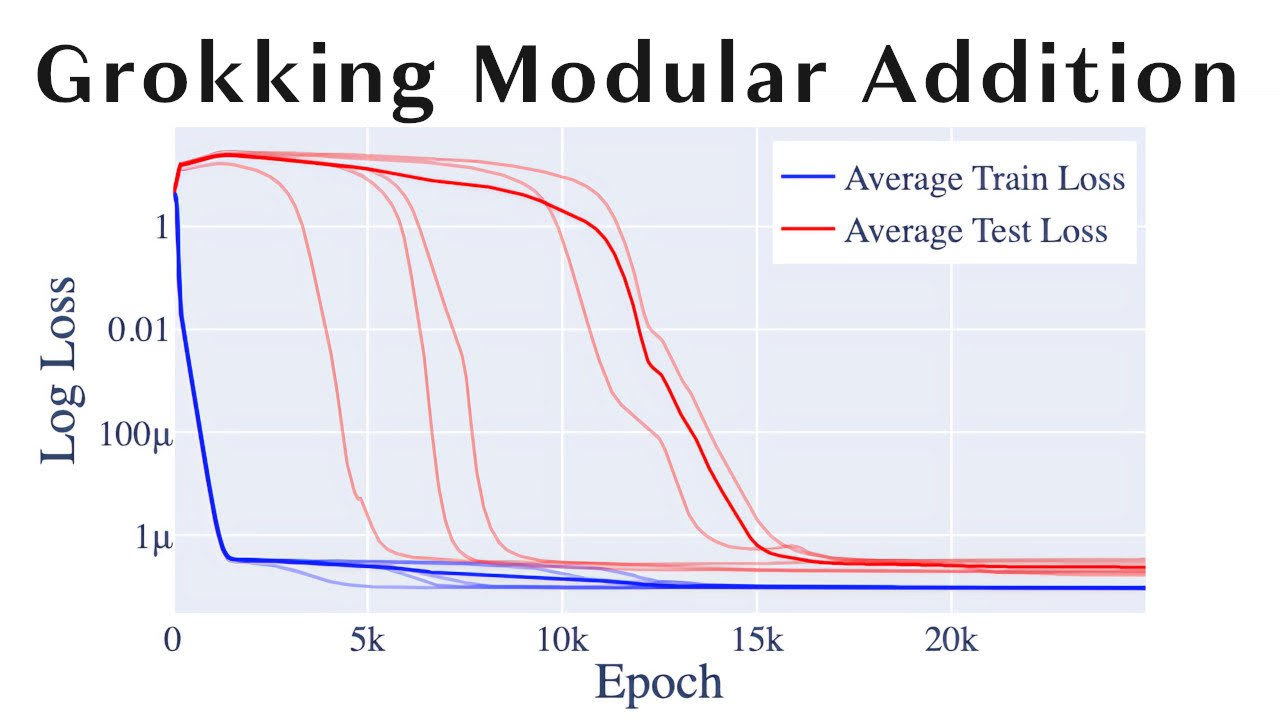
\includegraphics[width=.6\linewidth]{part1/visuals/Grokking_modular_addition.jpg}};
\begin{scope}[x={(plot.south east)},y={(plot.north west)},every node/.style={font=\scriptsize,inner sep=0pt}]
\fill[white] (0,.85) rectangle (1,1);
\node[font=\small] at (.50,.925) {模加法中的顿悟};
\fill[white] (0,.29) rectangle (.068,.66);
\node[rotate=90] at (.047,.475) {对数损失};
\fill[white] (.43,0) rectangle (.67,.08);
\node at (.55,.041) {训练轮次};
\fill[white] (.655,.72) rectangle (.885,.79);
\node at (.77,.755) {平均训练损失};
\fill[white] (.655,.65) rectangle (.885,.715);
\node at (.77,.682) {平均测试损失};
\end{scope}
\end{tikzpicture}
